\documentclass[12pt,a4paper]{article}

\usepackage[T1]{fontenc}
\usepackage{mathptmx}            % Times (Times New Roman style)
\usepackage[margin=1in]{geometry}
\usepackage{setspace}
\onehalfspacing                  % 1.5 line spacing
\usepackage{graphicx}
\usepackage{amsmath}
\usepackage{booktabs}
\usepackage{float}
\usepackage{xcolor}
\usepackage{listings}
\usepackage{enumitem}
\usepackage[colorlinks=true,linkcolor=black,urlcolor=blue,citecolor=black]{hyperref}
\usepackage{titlesec}
\usepackage{caption}
\setlist{itemsep=0pt,topsep=2pt,parsep=0pt}
\setlength{\parskip}{0pt}

\titleformat{\section}{\normalfont\bfseries\fontsize{14}{16}\selectfont}{\thesection}{0.6em}{}
\titleformat{\subsection}{\normalfont\bfseries\fontsize{12}{14}\selectfont}{\thesubsection}{0.6em}{}
\titlespacing*{\section}{0pt}{8pt}{3pt}
\titlespacing*{\subsection}{0pt}{5pt}{2pt}
\captionsetup{font=small,skip=3pt}

\lstset{
  language=Python,
  basicstyle=\ttfamily\fontsize{8}{9.2}\selectfont,
  commentstyle=\itshape\color[gray]{0.35},
  keywordstyle=\bfseries,
  frame=single, breaklines=true, columns=fullflexible, xleftmargin=0pt
}

\begin{document}

%================ TITLE BLOCK =================
\begin{center}
{\large\bfseries CSE 3207: Artificial Intelligence}\\[1pt]
{\Large\bfseries Understanding Bayes' Theorem and Na\"ive Bayes Classifier}\\[1pt]
{\normalsize\textbf{Name:} Samir Yeasir Ali \quad \textbf{ID:} 2203095 \quad \textbf{Date:} 14 November 2026}
\end{center}

%================ CHAPTER 1 =================
\section{Introduction and Background Study}

\subsection{Bayes' Theorem}
Bayes' theorem helps us to change our belief that was previously fixed after we get new information. First lets suppose we have some belief about a thing, for example ``this mushroom is poisonous''. Then we see some other information and evidence, for example the mushroom has a foul smell. Bayes' theorem tells us how we can update our first belief using that evidence \cite{russell2021}. The formula is
\begin{equation}
P(H \mid E) = \frac{P(E \mid H)\, P(H)}{P(E)}
\end{equation}
where $H$ is the hypothesis (for example, the class ``poisonous'') and $E$ is the evidence (the data we see). The four terms are:
\begin{itemize}
  \item \textbf{Prior, $P(H)$:} our belief about $H$ before seeing the evidence. In my dataset, 48.2\% of the training mushrooms are poisonous, so the prior of poisonous is 0.482.
  \item \textbf{Likelihood, $P(E \mid H)$:} how likely we are to see this evidence if $H$ is true. For example, how often a foul smell is found in poisonous mushrooms.
  \item \textbf{Evidence, $P(E)$:} how likely the evidence is overall, in all classes together. It makes all the probabilities add up to 1.
  \item \textbf{Posterior, $P(H \mid E)$:} our new belief about $H$ after seeing the evidence. This is what we want to find.
\end{itemize}

\subsection{How Na\"ive Bayes Comes from Bayes' Theorem}
In classification we have a data row with features $x_1,x_2,\dots,x_n$ and we want to find its class $C_k$. By Bayes' theorem,
\begin{equation}
P(C_k \mid x_1,\dots,x_n) = \frac{P(C_k)\,P(x_1,\dots,x_n \mid C_k)}{P(x_1,\dots,x_n)}
\end{equation}
The term $P(x_1,\dots,x_n \mid C_k)$ is very hard to find, because we have to see every possible combination of feature values many times. Na\"ive Bayes makes it easier with one assumption: given the class, every feature is independent of the others. So
\begin{equation}
P(x_1,\dots,x_n \mid C_k) = \prod_{j=1}^{n} P(x_j \mid C_k)
\end{equation}
The evidence in the denominator is the same for all classes, so it can be dropped when we only compare classes. The final rule is
\begin{equation}
\hat{y} = \arg\max_{k}\; P(C_k)\prod_{j=1}^{n} P(x_j \mid C_k)
\end{equation}
When every feature is a category (like ``odor = foul''), $P(x_j\mid C_k)$ is found by counting, and this version is called \textbf{Categorical Na\"ive Bayes} \cite{mitchell1997}. I used it in this assignment. In practice we add logarithms instead of multiplying, because many small probabilities multiplied together become too small for the computer.

\subsection{The ``Na\"ive'' Assumption}
The model is called na\"ive because it believes that when the class is known then the features do not affect each other. This is a very simple idea and many times it is not true. Some examples are:
\begin{itemize}
  \item In my own dataset, the colour of the stalk above the ring and the colour below the ring are the same in 62\% of the mushrooms, but the model treats them as two separate pieces of evidence.
  \item In text, words come together (``New'' and ``York''), and in medical data, tumor radius, perimeter and area are strongly connected.
\end{itemize}
When features are strongly related, the same information is counted many times, and the probabilities from the model become too extreme (too close to 0 or 1). But the predicted class is often still correct, because the model only needs to find which class has the highest score \cite{zhang2004}.

\subsection{Real-World Applications}
Na\"ive Bayes is fast, simple, and works well even with small data. It is used in: \textbf{spam detection} (email or SMS filters), \textbf{sentiment analysis} (positive or negative reviews), \textbf{disease prediction} (using symptoms and test results), \textbf{news and document categorization}, and \textbf{language detection}.

%================ CHAPTER 2 =================
\section{Dataset Description}

\subsection{Dataset Selection, Source and Details}
I have selected the \textbf{Mushroom} dataset from the UCI Machine Learning Repository \cite{schlimmer1987}. The records come from the \emph{Audubon Society Field Guide to North American Mushrooms} and describe 23 species of gilled mushrooms. I have selected it because all its features are categorical, it also has missing values, and the two classes are clear. I downloaded the same file (\texttt{mushrooms.csv}) from a public GitHub copy, and checked that its counts match the UCI description.

\begin{table}[H]
\centering
\caption{Summary of the dataset}
\begin{tabular}{ll}
\toprule
\textbf{Item} & \textbf{Value}\\
\midrule
Source & UCI Machine Learning Repository\\
Records (mushrooms) & 8,124\\
Features & 22 categorical (cap shape, odor, gill color, habitat, etc.)\\
Target variable & Class, with 2 classes: \emph{edible} (4,208) and \emph{poisonous} (3,916)\\
Missing values & 2,480 (all in the feature \texttt{stalk-root}, written as ``?'')\\
Duplicate rows & 0\\
\bottomrule
\end{tabular}
\end{table}

The two classes are nearly balanced (51.8\% edible, 48.2\% poisonous), so accuracy is a fair first measure here.

\subsection{Data Preprocessing}
\begin{enumerate}[label=\alph*)]
  \item \textbf{Missing values:} Only \texttt{stalk-root} has missing values, but it is 30.5\% of the rows, which is too many to delete. I kept ``?'' as its own category called \emph{missing}. As a second test, I also filled the missing values with the most common value (\emph{bulbous}) and compared both methods in Chapter 4. I also removed the column \texttt{veil-type}, because it has the same single value for every mushroom and so it gives no information. This left 21 features.
  \item \textbf{Encoding:} Every feature is categorical, so each category was changed into an integer code (for example, odor: almond $=0$, creosote $=1$, foul $=2$, \dots). The target was encoded as edible $=0$ and poisonous $=1$. I have taken \textbf{poisonous as the positive class}, because eating a poisonous mushroom is the dangerous mistake.
  \item \textbf{Normalization / standardization:} I was not used on purpose, because the integer codes are only labels, not real quantities. So mean and standard deviation have no meaning for them.
  \item \textbf{Train/test split:} I splited the data into 80/20 using a stratified split (fixed seed 42), so both parts keep the same ratio class. The training set has 6,499 mushrooms (3,366 edible, 3,133 poisonous) and the test set has 1,625 mushrooms (842 edible, 783 poisonous).
\end{enumerate}

%================ CHAPTER 3 =================
\section{Methodology}

I wrote the Categorical Na\"ive Bayes classifier from scratch using only Python, NumPy \cite{harris2020} and pandas \cite{mckinney2010}. Matplotlib \cite{hunter2007} and seaborn \cite{waskom2021} were used for plots only. The accuracy, precision, recall, F1-score, ROC curve and precision-recall curve were also coded by hand. The code is in \texttt{naive\_bayes\_mushroom.py} and is fully commented.

\textbf{Training.} For each class $c$ the model finds the prior $P(c)$, which is the number of mushrooms of that class divided by all mushrooms. Then, for each feature $j$ and each value $v$, it finds
\[
P(x_j=v \mid c)=\frac{\text{number of class-}c\text{ rows with } x_j=v \; + \;\alpha}{\text{number of class-}c\text{ rows} \; + \;\alpha K_j}
\]
where $K_j$ is the number of possible values of feature $j$ and $\alpha=1$ is the Laplace smoothing value. Smoothing is needed because a value that never appeared in a class would otherwise give probability 0 and make the whole product 0.

\textbf{Prediction.} For a new mushroom, the model calculates
$\log P(c)+\sum_j \log P(x_j\mid c)$ for each class, and the class
with the higher score is the prediction. Dividing by the sum over
classes (the evidence) gives the probabilities. The main part of the
code is given below, and the codes and scripts are also available on \\ GitHub:
\url{https://github.com/Samir0095/Mashroom_Detection}.

\begin{singlespace}
\begin{lstlisting}
class CategoricalNaiveBayes:
    def __init__(self, n_cats, alpha=1.0):
        self.n_cats, self.alpha = n_cats, alpha        # n_cats[j] = K_j

    def fit(self, X, y):
        self.classes_ = np.unique(y)
        self.log_prior_ = np.zeros(len(self.classes_))
        self.log_lik_ = [np.zeros((len(self.classes_), k)) for k in self.n_cats]
        for i, c in enumerate(self.classes_):
            X_c = X[y == c]                                   # rows of class c only
            self.log_prior_[i] = np.log(X_c.shape[0] / X.shape[0])
            for j, k in enumerate(self.n_cats):
                counts = np.bincount(X_c[:, j], minlength=k) + self.alpha  # count + alpha
                self.log_lik_[j][i] = np.log(counts / counts.sum())
        return self

    def log_posterior(self, X):                  # log P(c) + sum_j log P(x_j | c)
        out = np.tile(self.log_prior_, (X.shape[0], 1))
        for j in range(X.shape[1]):
            out += self.log_lik_[j][:, X[:, j]].T
        return out

    def predict(self, X):
        return self.classes_[np.argmax(self.log_posterior(X), axis=1)]
\end{lstlisting}
\end{singlespace}

The classifier was trained on the 6,499 training mushrooms (learned priors: edible 0.518, poisonous 0.482) and then used to predict the labels of the 1,625 unseen test mushrooms. To check my code, I ran scikit-learn's \texttt{CategoricalNB} \cite{pedregosa2011} on the same data. Its predictions were the same as mine for 100\% of the test mushrooms, and its AUC and average precision matched mine too. So my implementation was accurate. (scikit-learn was used only for this check.)

%================ CHAPTER 4 =================
\section{Results and Discussion}

\subsection{Part A: Model Evaluation}
TP = poisonous predicted as poisonous, TN = edible predicted as edible, FP = edible wrongly predicted as poisonous, FN = poisonous wrongly predicted as edible. The formulas are:
\begin{gather*}
\text{Accuracy}=\frac{TP+TN}{TP+TN+FP+FN}, \\ \qquad \\ \text{Precision}=\frac{TP}{TP+FP},\\ \\
\text{Recall}=\frac{TP}{TP+FN}, \\ \\ \qquad F_1=\frac{2\cdot \text{Precision}\cdot \text{Recall}}{\text{Precision}+\text{Recall}}
\end{gather*}

\begin{table}[H]
\centering
\caption{Confusion matrix on the test set (1,625 mushrooms)}
\begin{tabular}{lcc}
\toprule
 & \textbf{Predicted Edible} & \textbf{Predicted Poisonous}\\
\midrule
\textbf{Actual Edible} & 836 (TN) & 6 (FP)\\
\textbf{Actual Poisonous} & 66 (FN) & 717 (TP)\\
\bottomrule
\end{tabular}
\end{table}

\begin{table}[H]
\centering
\caption{Performance summary on the test set}
\begin{tabular}{lcccc}
\toprule
\textbf{Class} & \textbf{Precision} & \textbf{Recall} & \textbf{F1-score} & \textbf{Support}\\
\midrule
Poisonous (positive) & 0.9917 & 0.9157 & 0.9522 & 783\\
Edible & 0.9268 & 0.9929 & 0.9587 & 842\\
Macro average & 0.9593 & 0.9543 & 0.9555 & 1625\\
\midrule
\textbf{Accuracy} & \multicolumn{4}{c}{\textbf{0.9557 (95.57\%)}}\\
ROC AUC / Average precision & \multicolumn{4}{c}{0.9982 / 0.9981}\\
\bottomrule
\end{tabular}
\end{table}

\textbf{Discussion.} The model got 1,553 of 1,625 test mushrooms correct, which is an accuracy of 95.57\%. The training accuracy is 95.38\%, almost the same, so there is no overfitting. A silly model that always says ``edible'' would get only 51.8\%, so the model has really learned something. The precision for poisonous is very high (99.17\%): when the model says ``poisonous'', it is almost always right (717 of 723). But the recall for poisonous is lower (91.57\%): the model missed 66 of 783 poisonous mushrooms and called them edible. This is the most serious mistake in this problem, because a person could eat a poisonous mushroom. The 6 false positives are much less harmful, because a good mushroom is only thrown away.

\textbf{Making the model safer.} By default the model says ``poisonous'' when the score is above 0. I tried a lower cut-off ($-11.0$), chosen only from the training data (the lowest score of any poisonous mushroom in training), and then tested it on the test data. With it, the model found \textbf{all 783 poisonous mushrooms (recall 100\%, FN = 0)}, but it wrongly marked 153 edible ones as poisonous, so precision fell to 83.65\% and accuracy to 90.58\%. For a safety problem like this, that trade is probably worth it, but it is a choice that depends on how costly each mistake is.

\textbf{Is the result stable?} I also ran 5-fold cross-validation on the whole dataset. The accuracy of the folds was 95.57\%, 95.45\%, 94.95\%, 96.12\% and 94.58\%, so the mean is 95.33\% with a standard deviation of only 0.53\%. The result does not depend on one lucky split.

\textbf{Missing value methods.} Treating ``?'' as its own category gave 95.57\% accuracy and 91.57\% recall. Filling it with the most common value gave 95.63\% accuracy and 91.70\% recall. The difference is tiny (about 0.06 percentage points), so the method did not matter here.

\subsection{Part B: Result Visualization}
A \textbf{confusion matrix} is a table that compares the actual labels (rows) with the predicted labels (columns). The numbers on the diagonal are correct predictions and the numbers outside the diagonal are mistakes. Figure~\ref{fig:cm} shows it as a heatmap, and Figure~\ref{fig:dist} shows the distribution of actual and predicted labels.

\begin{figure}[!htbp]
\centering
\begin{minipage}{0.48\textwidth}
\centering
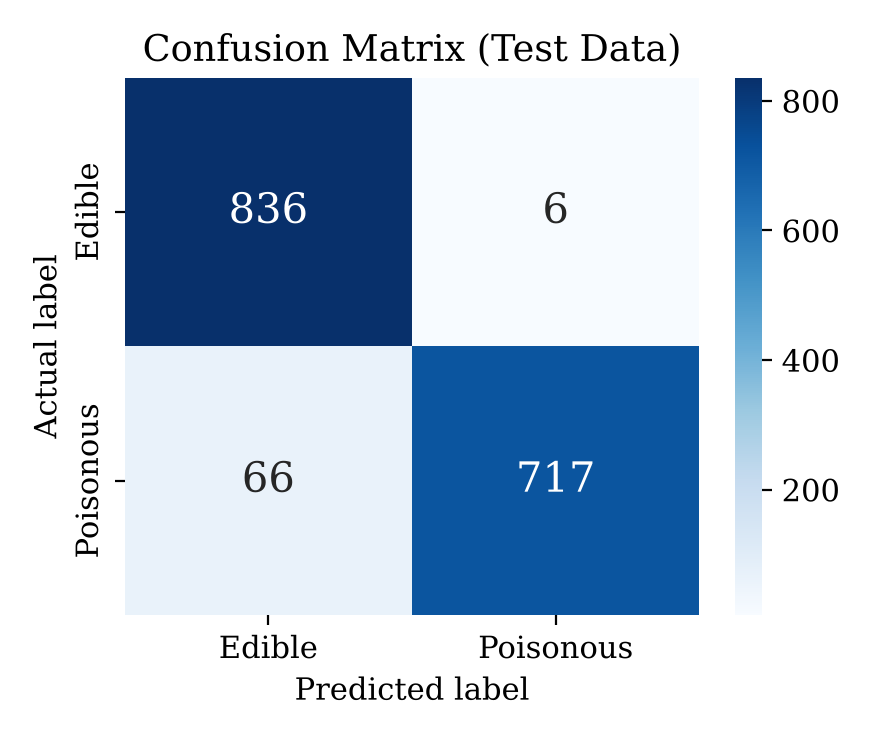
\includegraphics[width=0.74\linewidth]{confusion_matrix.png}
\caption{Confusion matrix of the test data}\label{fig:cm}
\end{minipage}\hfill
\begin{minipage}{0.48\textwidth}
\centering
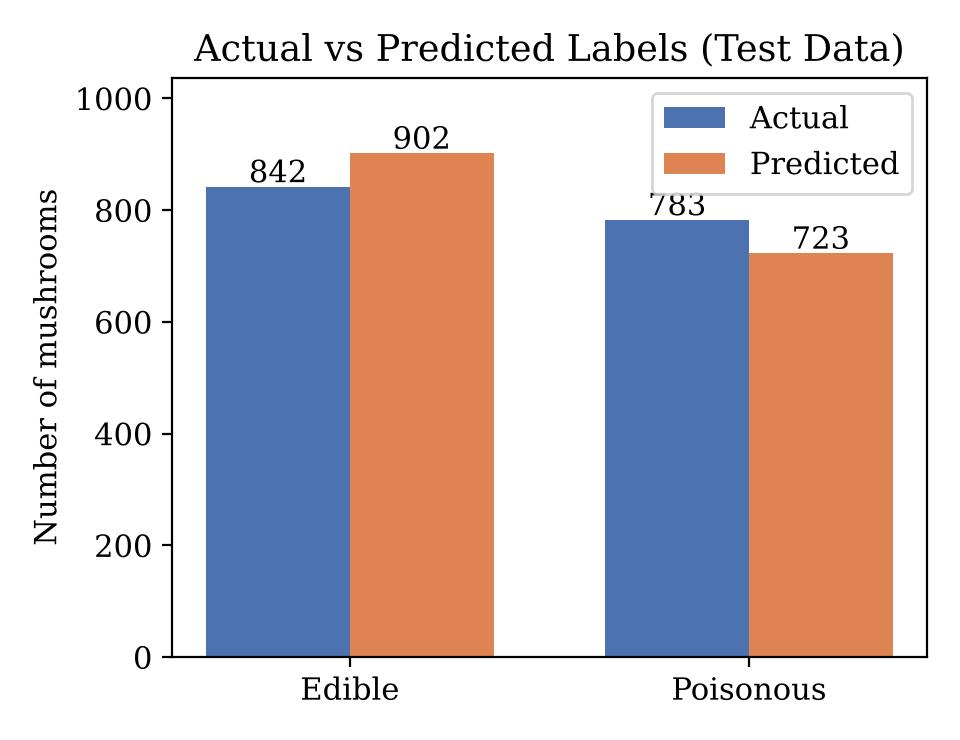
\includegraphics[width=0.74\linewidth]{label_distribution.png}
\caption{Actual vs predicted labels}\label{fig:dist}
\end{minipage}
\end{figure}

In Figure~\ref{fig:cm}, the dark boxes on the diagonal (836 and 717) are much bigger than the boxes outside (6 and 66). In Figure~\ref{fig:dist}, the real test set has 842 edible and 783 poisonous mushrooms, but the model predicted 902 edible and 723 poisonous. So the model says ``edible'' too often, and the 60 extra ``edible'' predictions are the missed poisonous mushrooms. This matches the high precision and lower recall for the poisonous class.

Figure~\ref{fig:summary} shows the performance summary as a chart (note that its vertical axis starts from 0.85 to make the differences easier to see). The green bars (edible) and red bars (poisonous) show the trade-off clearly: precision is highest for poisonous, and recall is highest for edible.

\begin{figure}[!htbp]
\centering
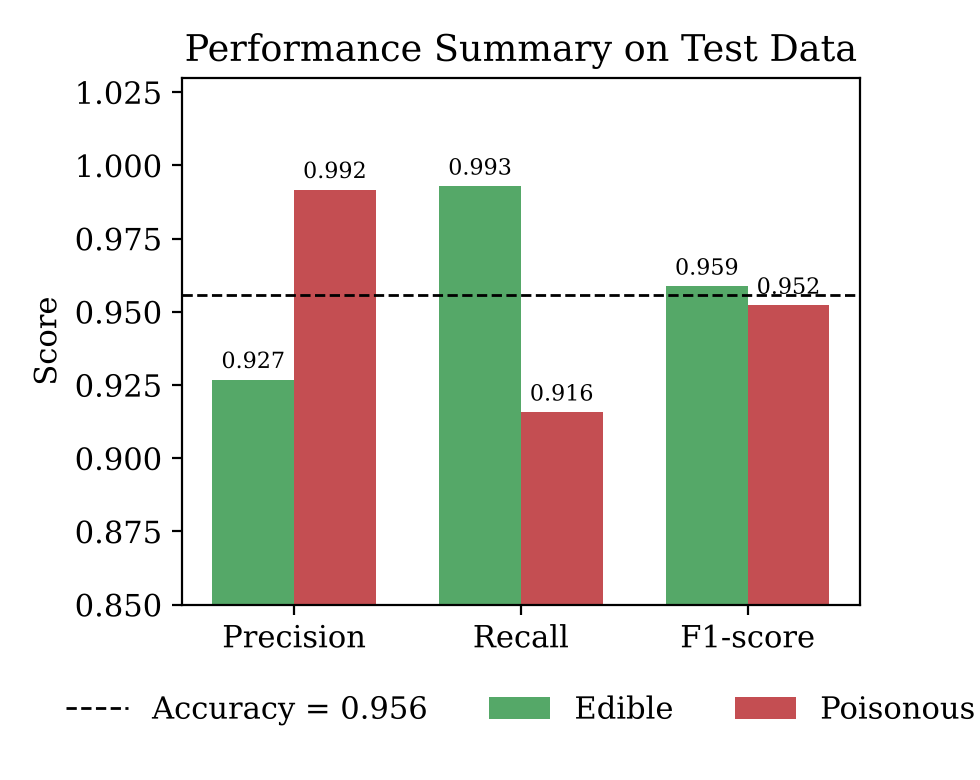
\includegraphics[width=0.38\linewidth]{metrics_summary.png}
\caption{Precision, recall, F1-score and accuracy}\label{fig:summary}
\end{figure}

The \textbf{ROC curve} (Figure~\ref{fig:roc}) plots the true positive rate (recall) against the false positive rate for every possible cut-off \cite{fawcett2006}. A curve near the top-left corner is good, and the area under it (AUC) is 1 for a perfect model and 0.5 for random guessing. My model has an \textbf{AUC of 0.9982}. The \textbf{precision-recall curve} (Figure~\ref{fig:pr}) plots precision against recall, and it is useful when we care about the positive class \cite{saito2015}. The average precision is \textbf{0.9981}. The black dot is the default cut-off, with high precision but recall of only 0.916. The curve shows that moving the cut-off to get full recall costs only a part of the precision, which is what we saw in the safer-threshold test.

\begin{figure}[!htbp]
\centering
\begin{minipage}{0.48\textwidth}
\centering
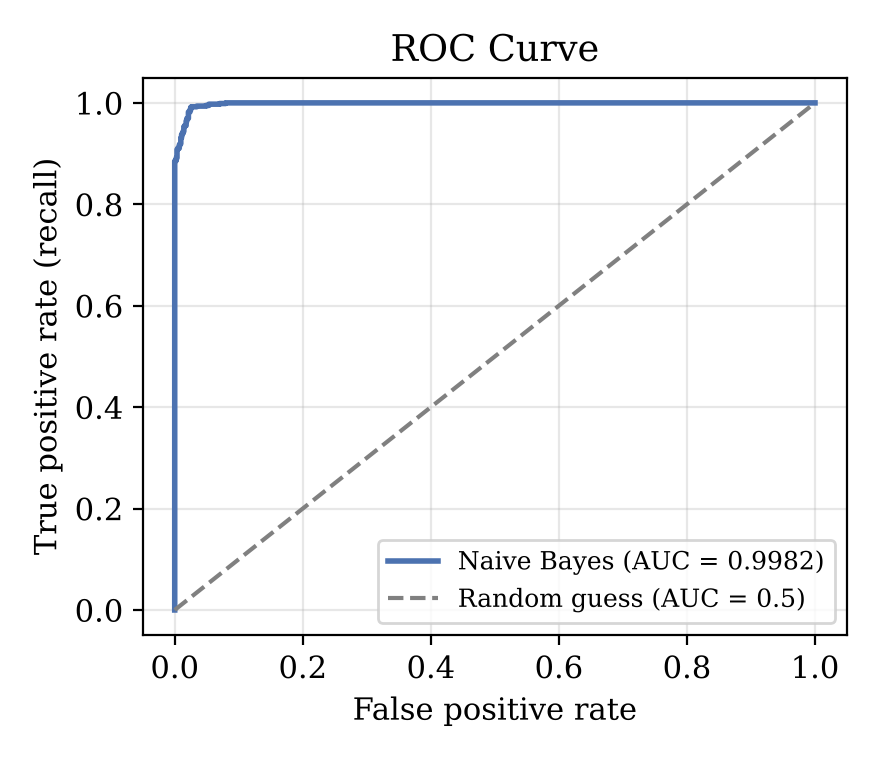
\includegraphics[width=0.74\linewidth]{roc_curve.png}
\caption{ROC curve}\label{fig:roc}
\end{minipage}\hfill
\begin{minipage}{0.48\textwidth}
\centering
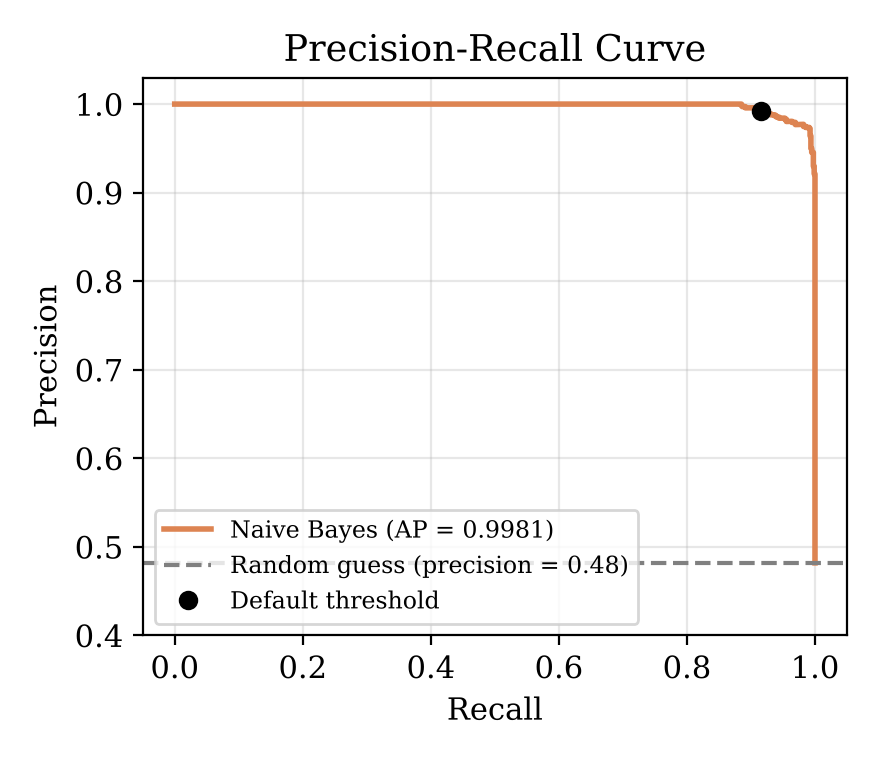
\includegraphics[width=0.74\linewidth]{pr_curve.png}
\caption{Precision-recall curve}\label{fig:pr}
\end{minipage}
\end{figure}

%================ CHAPTER 5 =================
\section{Conclusion}

In this assignment I have studied Bayes' theorem and how the Na\"ive Bayes classifier comes from it with the independence assumption. I built a Categorical Na\"ive Bayes classifier from scratch with NumPy and pandas and tested it on the Mushroom dataset. The main findings are:
\begin{itemize}
  \item The model reached \textbf{95.57\% accuracy}. For the poisonous class, precision was 0.9917, recall 0.9157 and F1-score 0.9522, with an ROC AUC of 0.9982 and average precision of 0.9981.
  \item Training accuracy (95.38\%) and test accuracy (95.57\%) are close, and 5-fold cross-validation gave $95.33\% \pm 0.53\%$, so the model is stable and does not overfit.
  \item The model missed 66 poisonous mushrooms (false negatives). A lower cut-off chosen from training data caught all of them, but it wrongly flagged 153 edible mushrooms.
  \item Keeping missing values as a category or filling them with the most common value gave almost the same result.
  \item My code gave the same predictions as the scikit-learn version, which confirms it is correct.
\end{itemize}
\textbf{Reflection.} I learned that accuracy alone is not enough: in a safety problem, the type of mistake matters more than the number of mistakes, and the ROC and precision-recall curves helped me to see the trade-off. Na\"ive Bayes was fast, easy to build, and good on categorical data, but its independence assumption is not true here (for example, the two stalk colors), and a model with 95.6\% accuracy still should not be trusted alone for deciding if a mushroom is safe to eat. In the future I can try removing repeated features, tuning $\alpha$ by cross-validation, and comparing with a decision tree or logistic regression.

%================ REFERENCES =================
{\setstretch{1.0}\footnotesize
\begin{thebibliography}{99}
\setlength{\itemsep}{0pt}
\bibitem{schlimmer1987} J. Schlimmer, ``Mushroom,'' UCI Machine Learning Repository, 1987. \url{doi.org/10.24432/C5959T}
\bibitem{russell2021} S. Russell and P. Norvig, \emph{Artificial Intelligence: A Modern Approach}, 4th ed., Pearson, 2021.
\bibitem{mitchell1997} T. M. Mitchell, \emph{Machine Learning}, McGraw-Hill, 1997.
\bibitem{zhang2004} H. Zhang, ``The optimality of Naive Bayes,'' \emph{Proc. 17th FLAIRS Conference}, 2004.
\bibitem{fawcett2006} T. Fawcett, ``An introduction to ROC analysis,'' \emph{Pattern Recognition Letters}, vol. 27, no. 8, pp. 861--874, 2006.
\bibitem{saito2015} T. Saito and M. Rehmsmeier, ``The precision-recall plot is more informative than the ROC plot on imbalanced datasets,'' \emph{PLoS ONE}, vol. 10, no. 3, e0118432, 2015.
\bibitem{harris2020} C. R. Harris et al., ``Array programming with NumPy,'' \emph{Nature}, vol. 585, pp. 357--362, 2020.
\bibitem{mckinney2010} W. McKinney, ``Data structures for statistical computing in Python,'' \emph{Proc. 9th Python in Science Conf.}, pp. 56--61, 2010.
\bibitem{hunter2007} J. D. Hunter, ``Matplotlib: A 2D graphics environment,'' \emph{Computing in Science \& Engineering}, vol. 9, no. 3, pp. 90--95, 2007.
\bibitem{waskom2021} M. L. Waskom, ``seaborn: statistical data visualization,'' \emph{Journal of Open Source Software}, vol. 6, no. 60, p. 3021, 2021.
\bibitem{pedregosa2011} F. Pedregosa et al., ``Scikit-learn: Machine learning in Python,'' \emph{J. Machine Learning Research}, vol. 12, pp. 2825--2830, 2011.
\end{thebibliography}}

\end{document}
